\documentclass{sig-alternate}

\usepackage{color}
\usepackage{cite}
\usepackage{float}
\usepackage{xspace}
\usepackage{amsfonts}
\usepackage{graphicx}
\usepackage{pgfgantt}
\usepackage{setspace}
\usepackage{gensymb}
\usepackage{pdfpages}
\usepackage{eurosym}
\usepackage{booktabs}
\usepackage{hyperref}
\usepackage[toc,page]{appendix}
\usepackage{multirow}

\hypersetup{
	colorlinks,
	citecolor=black,
	filecolor=black,
	linkcolor=black,
	urlcolor=black
}

\begin{document}

\title{Telemetry-based Optimisation for User Training in Racing Simulators}

\numberofauthors{1} 
\author{
	\alignauthor
	Fran\c{c}ois Buhagiar\\
    \email{francois.buhagiar.12@um.edu.mt}
}

\maketitle
\begin{abstract}

\end{abstract}

\keywords{Sim Racing, Motorsport Training, Serious Games}

\def \methodname {TeAR\xspace}
\def \methodnamefull {Telemetry Assisted Racing\xspace}

\section{Introduction}

\section{Background work} {
\label{sec:background}

In this section fundamental concepts relevant to this paper are given a brief overview. The section start by explaining what motor sports is and what is expected off a race drive. The section continues by mentioning fundamental concepts such as the racing line and how to achieve the limit of the car. An explanation of telemetry data is given and why it is important. The section concludes by explaining the differences between video games and serious games. 

\subsection{Motorsport Racing}
In circuit motorsport racing, motorised vehicles go round a course for a set number of times. There are varies racing disciplines or series, each one having its own specific rules. However, at the core, participants in all disciplines aim to complete a full lap of the circuit in the shortest time. This paper will focus on one such discipline, that of confined car racing, which takes place on smooth asphalt surfaces in purpose-built race tracks in which the aim is to perform the fastest lap possible. 

\begin{figure}[!htb]
	\centering
	\begin{minipage}{0.45\textwidth}
		\centering
		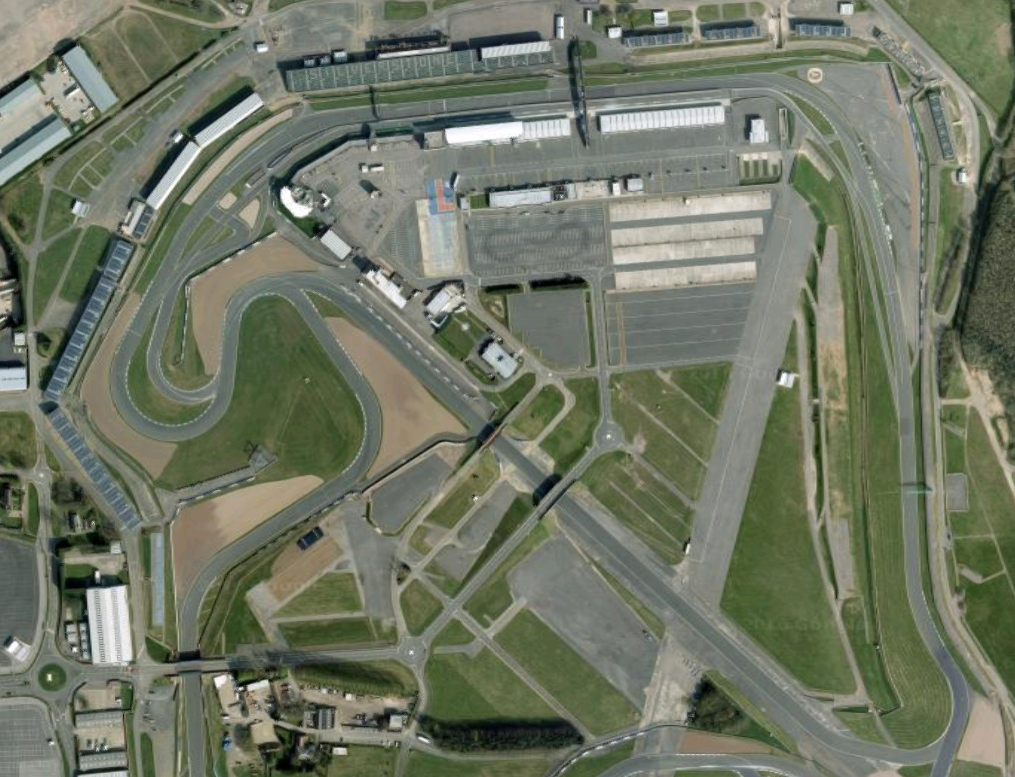
\includegraphics[width=\textwidth]{images/confinedCircuit}
		\caption{Example of confined car racing circuit}
		\label{fig:circuit-overhead}
	\end{minipage}\hfill
\end{figure}

\subsection{Racing Line}
\emph{A race driver needs to figure out how to go round a piece of asphalt in the minimum amount of time} \cite{GoingFaster}. In order to do so, he or she needs to develop techniques for more advanced vehicle control. One such technique is that of mastering the racing line, which is considered the fundamental skill a race driver must understand and master before moving on to anything else \cite{GoingFaster}. The racing line is the best path through a circuit: if followed, it is the path that yields the shortest time at the highest average speed \cite{beckman1991physics}. The trickiest part in achieving this is to master the racing line of a corner. Corners are split in three sections. The first section is the breaking part, where the car needs to sufficiently decelerate in preparation for the  \emph{turn-in point}. Thus, the second partition of the racing line at a corner is the segment between the turn-in point and the apex point, which is the inside mid-point of the corner (see Figure \ref{fig:CornerRaceLine}). After the turn-in point, the driver aims for the apex point. The final section of the racing line in a corner lies from the apex point onwards, where the driver must gradually accelerate out of the corner, while still turning, aiming for the outside apex (see Figure \ref{fig:CornerRaceLine}.

\begin{figure}[!htb]
	\centering
	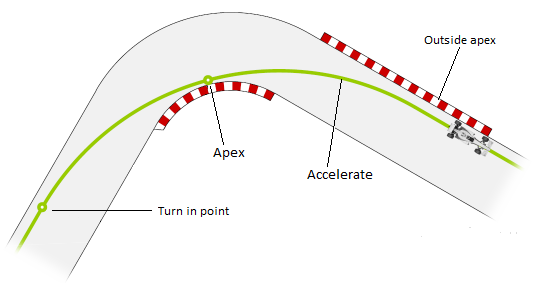
\includegraphics[width=0.45\textwidth]{images/cornerraceline}
	\caption{Racing line through a 90" right corner}
	\label{fig:CornerRaceLine}
\end{figure}

\subsection{Limit Of The Car}
After the driver develops a good grasp of the racing line, the limit of the car must be found. This is the highest speed the car can be driven while still retaining some measure of control. Various studies have been carried out to define such a limit in terms of the physical properties of the car and its environment \cite{beckman1991physics}. The most important property is the level of grip the car can achieve and sustain on track. A number of factors contribute to the level of grip. Most notably, one very important factor is the tyres as they are the only contact the car makes with the track, and allow for braking, accelerating and turning forces to be transferred to the asphalt.

Each tyre has two properties which are of particular interest: the slip ratio and slip angle. The slip ratio refers to the level of slip occurring between tyre rotational velocity and the asphalt which occur during acceleration and deceleration The \emph{slip ratio} is expressed as a percentage: a slip percentage of 100\% means that the tyre is rotating but the road is stationary. In jargon, this is called \emph{wheel spin}. On the other hand, a percentage of -100\% indicates that the tyre is not rotating but the road beneath is moving. This can occur when braking too hard and is called \emph{locking the wheels}. Both events need to be avoid by the driver as they not only put excessive wear and tear, they also impact negatively the performance of the driver. For an optimal braking procedure, the slip ratio should be between 10\% to 15\% \cite{GoingFaster} and no slip should occur during acceleration.

The slip angle is the angle between the tyre's desired direction (perpendicular to the axis of rotation of the tyre) and the tyre's actual direction (the direction the car is moving in). Given both the actual direction of travel ($\mathbf{d}_t$) and the desired direction ($\mathbf{d}_d$) are known, the slip angle $s_a$ is calculated as follows:
\begin{equation}
s_a = \cos^{-1}(\hat{\mathbf{d}}_d \cdot \hat{\mathbf{d}_t}),
\end{equation}
\noindent where $\hat{\mathbf{d}_d} = \frac{\mathbf{d}_d}{|\mathbf{d}_d|}$ and $\hat{\mathbf{d}_t} = \frac{\mathbf{d}_t}{|\mathbf{d}_t|}$ are the normalised direction vectors for desired and travel directions respectively.

Whenever the slip angle is above $0\degree$ ($s_a > 0$) the tyre is said to be in an understeering situation. Understeer can be caused by active factors such as cornering speed, throttle application, braking, steering inputs and weight transfer. A tyre has an optimal slip angle at which grip is maximised during cornering. The optimal slip angle for a road tyre is about $5\degree$, whereas for a slick tyre, which is purposely constructed for racing, is about $8\degree-10\degree$ \cite{beckman1991physics}.

An oversteering situation may arise from lack of grip; while understeer is caused by a lack of grip in the front tyres, oversteer is cause by a lack of grip on the rear tyres. Oversteer is usually denoted by the rear of the vehicle becoming unstable resulting in its rotation such that the driver is facing towards the inside of the corner. Similarly to understeer, the active factors causing oversteer are also cornering speed, throttle application, braking, steering inputs and weight transfer. Oversteer is usually induced by braking during a corner or accelerating too hard in a rear wheel drive vehicle.

\subsection{Telemetry Data}
In motorsport, telemetry data contains measurements of vehicle dynamics from the engine and other components and is transmitted to receiving equipment for remote monitoring. These measurements can serve to monitor and reconstruct the vehicle state at a particular point in time. Telemetry data in motorsports usually accounts for measurements of speed, engine speed, component temperatures, slip angles, slip ratios, etc. Telemetry is widely regarded as the most important source of information by motorsports engineers; analysing this data can lead to a better understanding of the respective strengths and weaknesses of the car and the driver \cite{CarDataAnalysis}. In this work, we posit that through the real-time analysis of telemetry data, the pedagogical aspect of sim racing can be exploited to teach race driving to non experts.

\subsection{Racing Simulation Rigs}
The racing simulation rig (sim racing rig) is a piece of equipment designed to mimic the cockpit of a real-world car. The quality of a sim racing rig is dependent on its authenticity - how similar it is to a real-world car - and its build quality. These rigs come in various shapes, forms and sizes, from hangar-sized hydraulic-driven car chassis, that cost millions of Euro, to the more modest, built from off-the-shelf commodity hardware. Minimally, a rig should provide a steering wheel, seating and a display. More sophisticated rigs augment the user experience by employing gear shifters, and clutch, throttle and breaking pedals. The more advanced components are furnished with a force feedback mechanism, a form of haptic technology used to replicate the sense of touch by applying forces or vibrations, or motions to the user \cite{li2015can}.

\subsection{Video Games and Serious Games}
The main contrast between video games and serious games is the use of pedagogic activities which aim to educate or instruct knowledge or skill \cite{zyda2005visual} in serious games as opposed to the pure leisurely aspects of the video game. Pedagogy is given preference over the amusement value which in some cases might not be found in serious games \cite{zyda2005visual}. Serious games need to educate the player with a specific type of content, whereas videos games need to entertain the player with whatever; racing, puzzles, it does not really matter, as long as the player enjoys it\cite{Harteveld2007}. On the other hand, serious game designers have multiple objectives, they still need to create a compelling and fun game, but also an educating and realistic game. From this it follows that three aspects as essential for a serious game, fun, learning and validity \cite{Harteveld2007}. The serious game should make use of pedagogical methods and theories to ensure knowledge can be conveyed.
}
\section{Methodology}
\label{sec:Methodology}

\section{Design and Implementation}

\section{Evaluation} {
\label{sec:Evaluation}

In this section findings from the user study are presented. The section start by describing the hardware setup used for the experiments followed by an overview of the participants' demographic. Experiments results are presented showing the resulting dataset for the laptimes and the outcome of the statistical analysis. Participants' feedback is presented and the section concludes with a discussion resulting from the findings.

\subsection{Experiment Setup}
The user study has been carried out in line with the methodology described in Section \ref{sec:Methodology}. The sim racing rig framework was custom-built, and the Logitech G25 input devices mounted on it. The display device used was a 32" LCD HD Samsung monitor also capable of outputting stereo audio from 2x10W speakers. The racing simulator used in this experiment is Assetto Corsa by Kunos Simulazioni, running in full HD resolution at 60 frames per second (fps). The hardware platform running the simulator is an Intel Core i7-940, with 8GB of RAM and an Nvidia 660Ti video card with 2GB VRAM. The machine is running the retail version of the Windows 10 Professional operating system.

\begin{figure}[!htb]
	\centering
	\begin{minipage}{0.45\textwidth}
		\centering
		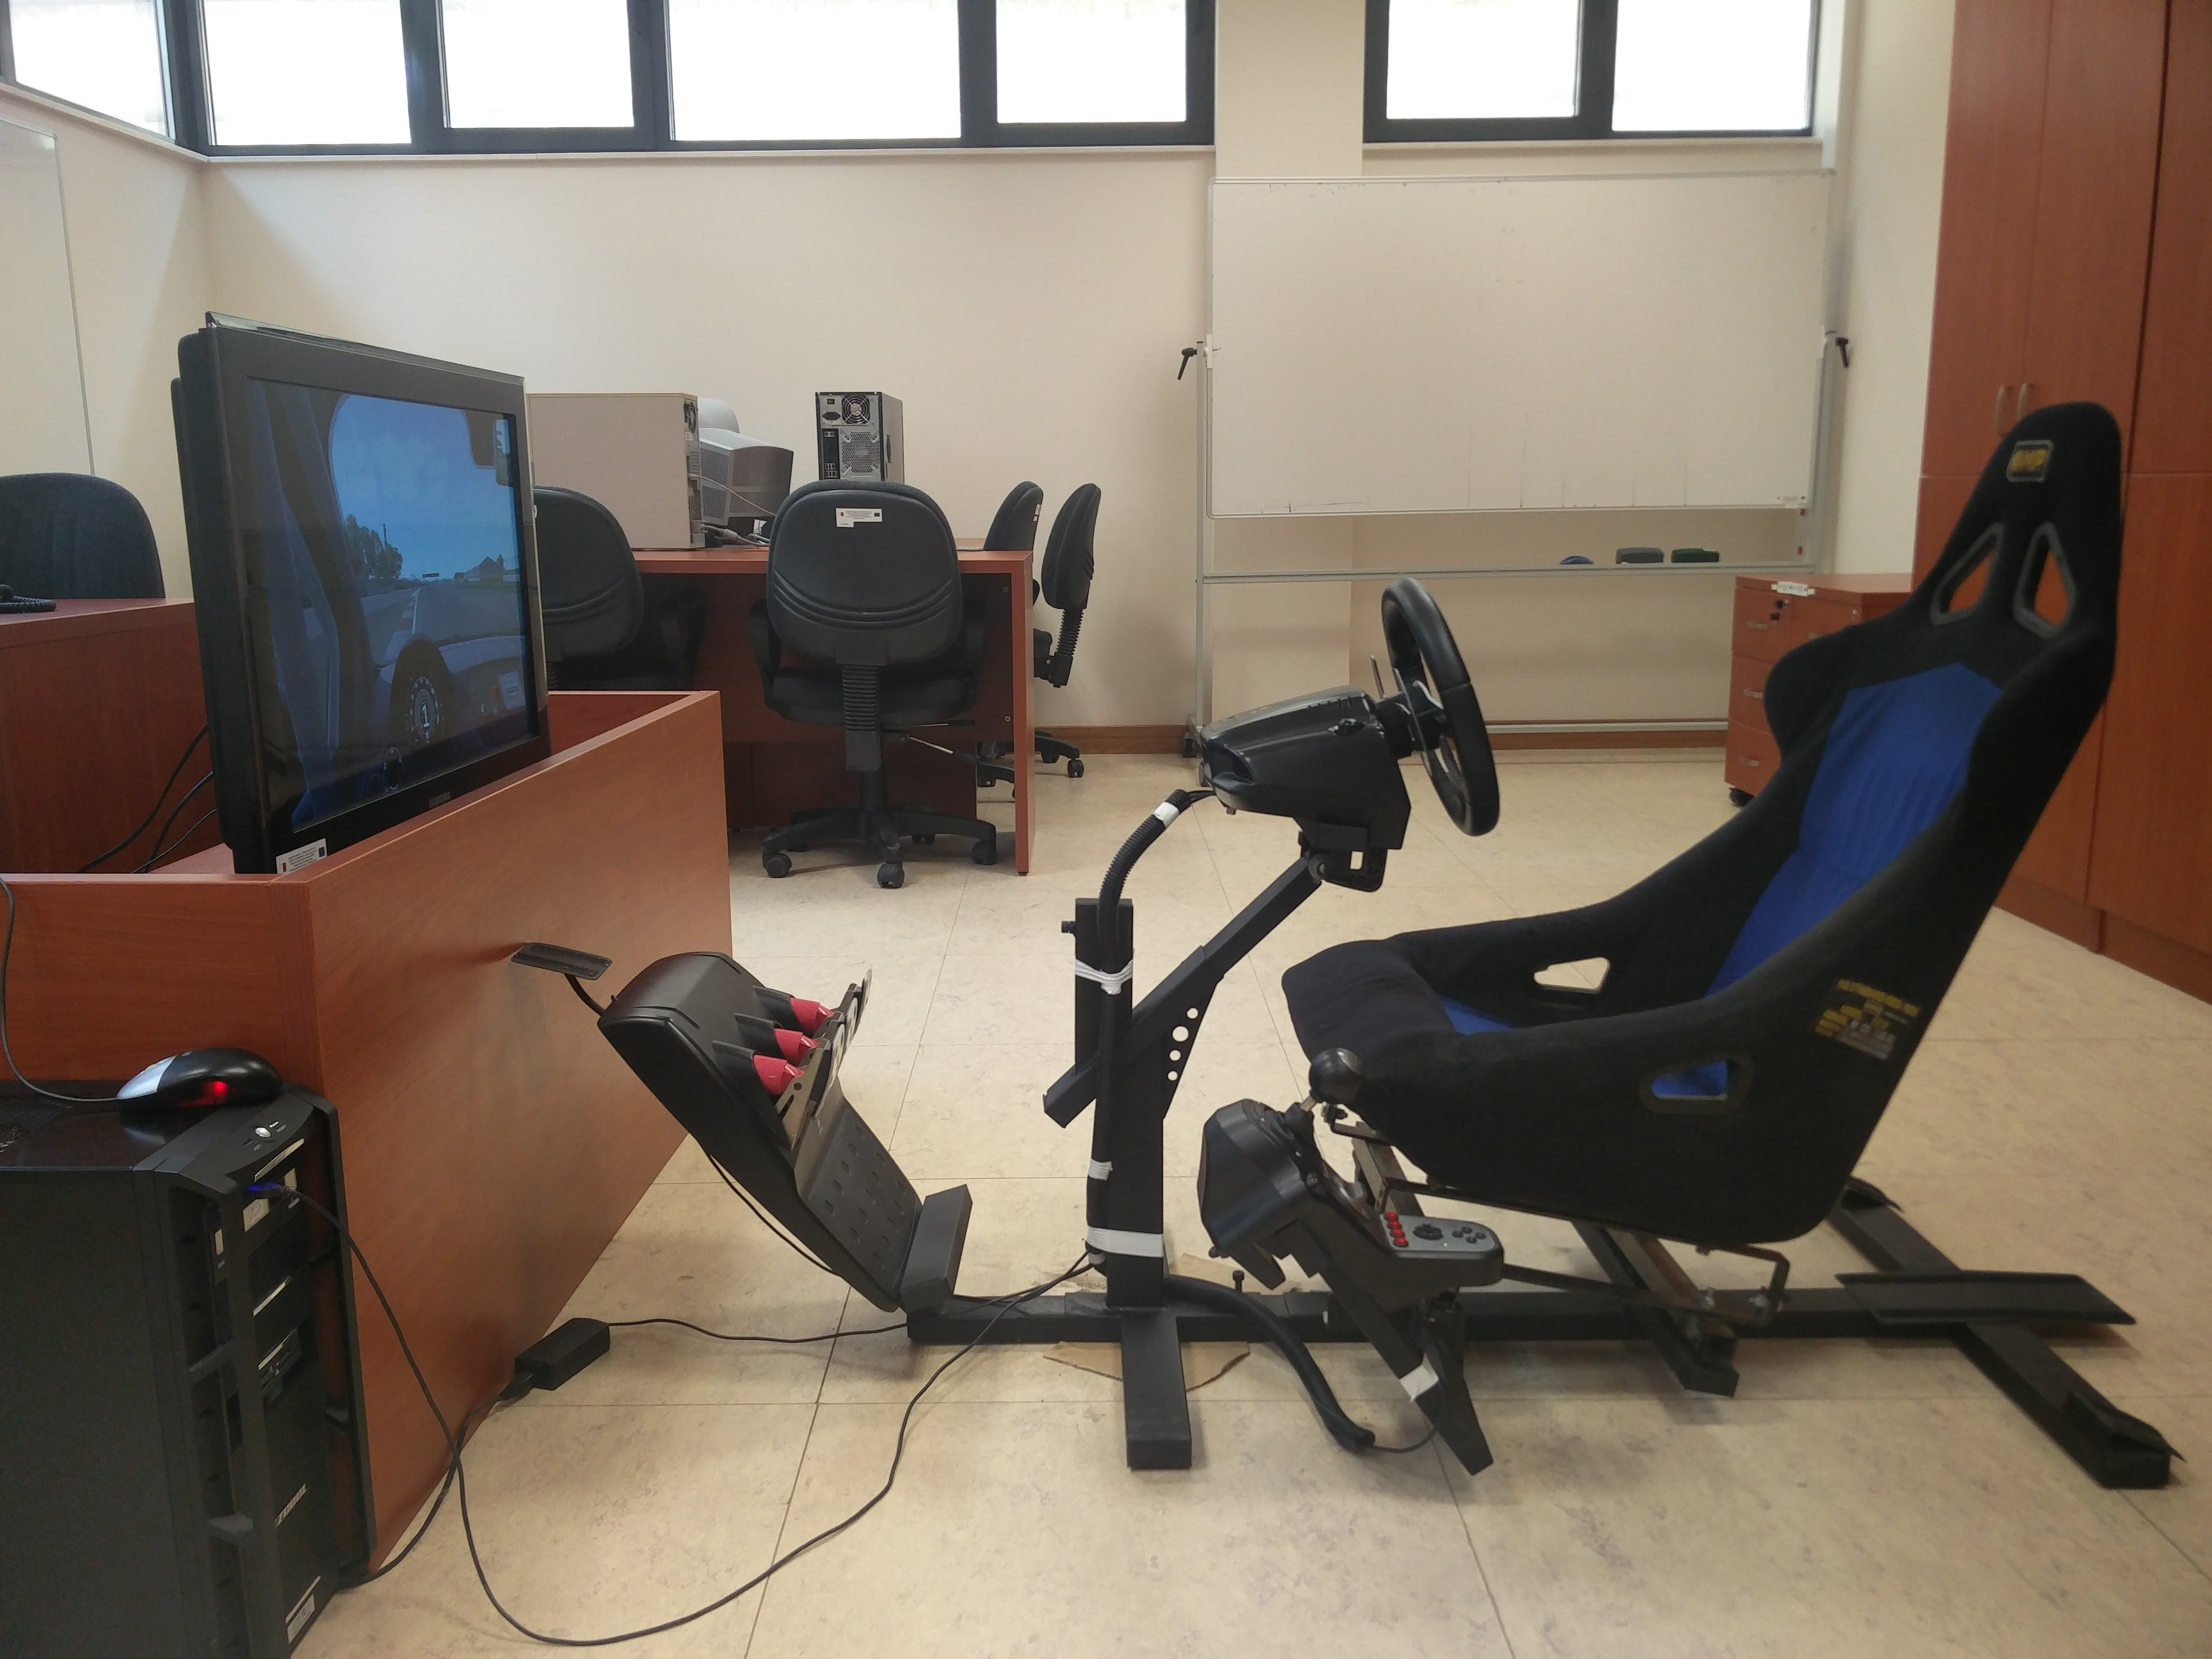
\includegraphics[width=\textwidth]{images/RacingRig}
	\end{minipage}\hfill
	\caption[Side view of the racing rig]{Side view of the racing rig}
	\label{sec:eval-simRacingRig}
\end{figure}

\subsection{Sample Demographic}
During the experiments, 27 participants took part most of which were males in their early twenties. Out of 27 participants, 2 did not hold a driving license; 25 had a driving license, although most of them haven't been driving for more than a year. 22 participants claimed to play video games, from which 18 stated to have played racing video games. Out of these 18, a majority of 15 play mostly arcade sim racing games, while the remaining 3 regularly play simulation racing games. 7 out of 27 participants have previously used a racing rig. Random assignment was used to split the participants into the control and feedback/experimental group. The control group had 13 participants, while the feedback group had 14.

\subsection{Experiments Results}

\begin{figure}[!htb]
	\centering
	\includegraphics[width=0.45\textwidth]{charts/laptimes.png}
	\caption[Lap times vs session, clustered by group]{Blue : Control Group, Green : Feedback group \\ Lap times vs session, clustered by group}
	\label{fig:chart-laptimes}
\end{figure}

The dataset of the 1st session shown in Figure \ref{fig:chart-laptimes} was subjected to the Kolmogorov-Smirnov Test; the result had a p-value of 0.360, with a significance level of 0.05 the null hypothesis is accepted. The groups share the same distribution, hence the Mann-Whitney U Test can be used.

\begin{table*}
	\centering
	\begin{tabular}{|l|l|l|l|l|}
		\hline
		& \multicolumn{4}{c|}{LapTime}            \\ \cline{2-5} 
		& 1st Session & 2nd Session & 3rd Session & 4th Session \\ \hline
		Asymp. Sig. (2-tailed) & .057 & .054        & .029        & .539        \\ \hline
	\end{tabular}\\
	Grouping Variable : Group
	\caption[Mann-Whitney U Test for Experiments' Sessions]{Mann-Whitney U Test result for Experiments' Sessions}
	\label{table:Mann-Whitney-Sessions}
\end{table*}

The Mann-Whitney Test is used to determine differences in the groups. The results of the test are shown in Table \ref{table:Mann-Whitney-Sessions}. For the first session these show a p-value of 0.057, with a confidence interval of 0.95 resulting in no statistical difference between the groups (p-value $> 0.05$, thus accepting the alternative hypothesis).  The tests for the second and fourth session have a p-value of 0.054 and 0.539 respectively; both values are above the significance level of 0.05, resulting in the alternative hypothesis being accepted. The third session, however, has a p-value of 0.029, resulting in accepting the null hypothesis suggesting there is statistical difference in the groups' performance.

\subsection{Participant Feedback}
The participants reported a good experience overall. The rig setup was found to be realistic and easy to use. With respect to the difficulty of the race track, an overwhelming majority of the respondents reported having issues mastering the second and third corners (referred to as the \emph{s-bend}). When the feedback group was asked about \methodname, they reported the feedback and the output quality of the audio to be intelligible, accurate and helpful. They also said that the feedback hints were somewhat easy to apply. Lastly, when asked whether the feedback was intrusive and possibly distractive, 10 out of 14 respondents reported that it was neither intrusive nor distractive.

\subsection{Discussion}
The rig setup has been well received, with participants enjoying the driving and awarding it a high score in terms of realism. This suggests that is it possible to achieve a good level of realism using simple off-the-shelf hardware. 
Both groups show a noticeable improvement from one session to the next, except for the final session in which the shorter time slot allocated might have put additional pressure on the participants, hindering their performance.
For the second session, the tests shown no statistical differences in the performance of the two groups, albeit this changed for the third session. The lower average lap time for the feedback group suggests that after familiarising with the feedback system, the group started following its instructions more closely, thus improving their performance.

The available sample of participants is too small to test for correlation between gaming experience and lap times, The same argument can be made for a possible correlation between holding a driving licence and driving performance, since all but two participants are in possession of a driving licence.
}

\section{Conclusions} {
\label{sec:Conclusions}
The skills required to become a good motorsport driver are generally learned through practice, and suggestions provided by more experienced drivers. Our hypothesis for this work is that an automated telemetry-based feedback system can be used to simulate this process and thus, to possibly help novice drivers assimilate this knowledge at a higher rate. For this purpose, \methodname was developed, which using a static expert system, presents auditory suggestions to drivers underlining the driving mistakes they are currently making. An was set up to verify this hypothesis with 27 participants taking part. From the data gathered in this experiment, it appears that the real-time feedback was effective to some extent; however, the participants seemed to be having difficulty retaining and applying the suggestions once it was switched off. This lack of cognitive retention may be due to a number of reasons, which could be investigated in future work.

\subsection{Future Work}
At present, \methodname presents feedback only when the driver is performing something wrong. It would be interesting to determine whether a system which also presents positive feedback, for instance letting the driver know that a previously reported mistake was actually corrected, would lead to any improvements. Furthermore, it is also possible to experiment with a variety of feedback methods, both visual and auditory, on the assumption that different feedback presentation media can lead to changes in the learning rates. Combining both auditory and visual feedback could help in increasing the clarity of the feedback provided. The feedback mechanism of \methodname is entirely based on telemetry data provided by the racing simulation software. However, a number of mistakes cannot be directly extracted from this data. For instance, during the experiment it was noted that some of the participants lacked some basic driving skills such as keeping both hands on the steering, not crossing hands while steering and not resting hands on the shifter. This additional information could be collected through the use of a motion tracking camera which directly feeds \methodname.   

\methodname is currently intended to help drivers improve their motorsport driving skills. A future direction could also look into the possibility of using \methodname to automate the driving process of a racing car. One possibility is that of using neural nets and fuzzy logic controllers, with both models learning how to drive via the feedback provided by \methodname.

}

\bibliographystyle{abbrv}
\bibliography{sigproc}

\end{document}
